\chapter{General-Purpose Computing on Graphics Processing Units}
General-Purpose computing on graphics processing unit (GPGPU) is the utilization of graphics processing unit (GPU), which was originally designed for computer graphical computations, to cooperate with central processing unit (CPU) on general tasks which are normally processed only by CPU.\\
Because solving graphical tasks require many vector or matrix computations, which are naturally parallel, GPU's architecture contains many simple cores capable of basic mathematical operations and parallel work. This is their main advantage in comparison with ordinary CPU - they have ten times, a hundred times but lately thousand times more cores designed to work in parallel, so if the task is well parallelizable, it could be accelerated up to hundred times on GPU in comparison to serial CPU version.\\
At the beginning of GPGPU, cards support only computation of vectors or matrices, usually two, three or four dimensional because these structures are commonly used in graphics computations, so general purpose computation had to be reformulated to this graphical principles supported by major graphics APIs like DirectX or OpenGL. This transformation was hard for programmer and very often impossible, so many algorithms could not be transfered to graphical problems and could not be parallelized on GPUs.\\
This problem disappears later with the arrival of specialized frameworks for utilizing GPUs for general purpose programming. These frameworks allows to programmer hides limitations of graphics environment and make general computations easier.~\cite{Kirk12}\\
Nowadays there exist two major frameworks for GPGPU - CUDA~\cite{Sanders10} and OpenCL~\cite{Scarpino11} (open computing language). The main advantage of CUDA is a direct link to the hardware, which is not the case of OpenCL and others. This is because CUDA is developed by Nvidia and only for Nvidia graphics cards so it could use concrete hardware specific properties. Compared to that, OpenCL by Khronos group is a universal, vendor independent framework for parallel computations supporting a large range of hardware divergent devices - it can be run on many CPUs and GPUs including Nvidia. This wide support of devices is a problem for high performance computing because OpenCL could not use every property of concrete architecture and hardware simply because there is nothing like concrete architecture. In the opposite CUDA is designed only for cards by Nvidia so it benefits from a small range of supported devices. In this work, we decided to use CUDA for one of the best performances among other frameworks and because we will not take main OpenCL advantage, the portability.\\
Other advantage of CUDA is that the device code and host code are written together and that they are both compiled in compile time in difference to OpenCL which compile device code at runtime.

\section{GPU architecture}
GPU is multi-processor highly tuned for graphics which demands fast processing of many floating point operations. Physically, it could be placed on special graphical card connected to mother board usually by PCI Express bus or it could be placed directly on CPU chip. Because GPUs integrated into CPU are not so powerful, we will focus on external graphical cards. Directly on graphical card are GPU chip and also memory to reduce memory latency. GPU usually consists of following components:
\begin{description}
\item[unified shaders] are programmable execution units responsible for computations. They replaced specialized shaders like vertex shaders or pixel shaders. Due to unification, the workload could be better balanced and for example tasks with many geometry computations, system can allocate most computing units for geometry shaders. Because of unification, also non-graphical tasks could be computed on GPUs.
\item[memory controller] is responsible for communication between GPU and graphical memory.
\item[texture mapping unit] is placing textures on objects
\item[render output unit] makes the final image sent to output device.
\end{description}
For GPGPU computations, only unified shaders and memory (memory controller) is used.

\subsection{GPU and CPU comparison} \label{ssec:gpucpucomparison}
Main difference between CPU and GPU is in their specialization. Instead of general purpose of CPUs, GPUs are specialized on graphics. Graphical computations requires high throughput of data, so their architecture is targeted for massive parallel calculations with numbers. The single cores are significantly different too because CPU core usually works on higher frequency (about 2 - 3 GHz) and supports many instructions in comparison to GPU core which works on lower frequencies (800 - 1000 MHz) and supports only special set of instructions. Problem was the special designation of GPUs but after GPGPU was introduced, problem with GPU specialization was solved by special frameworks and GPUs began to compete with processors. Main differences between CPUs and GPUs are:
\begin{description}
\item[Number of cores] CPU has only few physical cores~\autoref{fig:cpuarchitecture}. Common CPUs have up to 8 logical cores, server CPUs could have more, but usually it is between 8 and 12 cores on chip. Compared two that, modern GPUs have around thousand CUDA cores~\autoref{fig:gpuarchitecture}, the top models have thousands of cores (for example, GeForce GTX Titan X has CUDA cores), so they have great potential for parallel tasks.
\item[Core architecture] GPU cores are specialized for numeric computations, not for general tasks as CPU cores. This is not so big limitation of GPU, because the are usually used for numeric computations. CPU advantage is frequency, usually, CPU core is five times faster than GPU core. But because of specialized optimizations, which allows certain calculations to go much faster than on CPU, lower frequency is not a problem. The lesser frequency of GPU has several reasons, for example it is really hard to take away heat generated by thousands of cores placed on single chip and  because higher frequencies generates more heat, GPU can not run on faster frequencies like CPU.
\item[Threads] Approach to threads is also different. CPU can process different instructions at one time, which is called Simultaneous Multithreading (SMT), GPU multiprocessor is capable of running multiple threads, but with same code, because execution units shares single fetch/decode unit.
\item[Memory] CPUs use big cache memory for hide latency of memory access so when thread is switched to different core, there is problem with locally cached data, which could be useless (depend on cache type) on original core and must be re-cached on new core. GPU has only smaller caches, but the threads are not switched between cores.
\end{description}

\begin{figure}[h]
\centering
\begin{subfigure}{.49\textwidth}
  \centering
  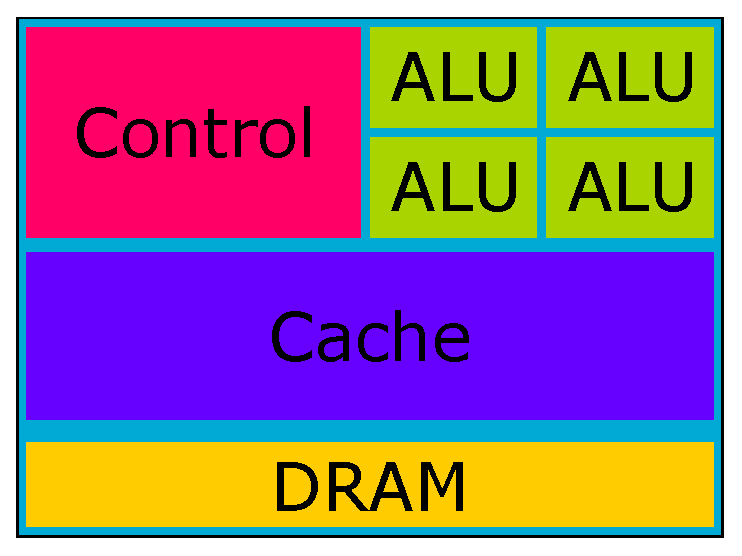
\includegraphics[width=1\linewidth]{img/CPUarchitecture.eps}
  \caption{CPU architecture}
  \label{fig:cpuarchitecture}
\end{subfigure}
\begin{subfigure}{.49\textwidth}
  \centering
  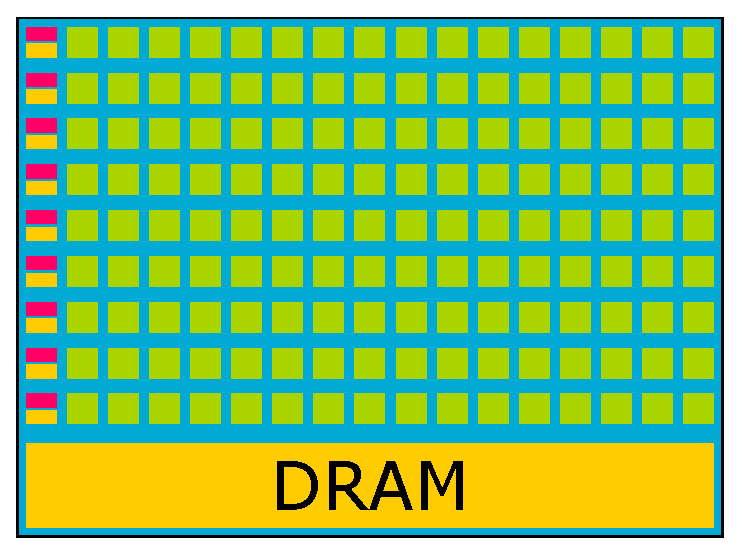
\includegraphics[width=1\linewidth]{img/GPUarchitecture.eps}
  \caption{GPU architecture}
  \label{fig:gpuarchitecture}
\end{subfigure}
\caption{CPU and GPU architecture comparison (same colors of boxes in GPU means same units)}
\end{figure}

%\begin{table}
%\begin{tabular}{|l|l|l|}
%\cline{1-2}
%NIC & CPU & GPU \\ \cline{1-2}
%# cores & Few cores per chip & Many cores per chip \\ \cline{1-2}
%Specialization & General purpose cores & Cores psecialized for numeric computations \\ \cline{1-2}
%Threads approach & Processing different threads & SIMT thread processing \\ \cline{1-2}
%Memory access & Huge caches to reduce memory latency & Huge amount of threads and fast context switch \\ \cline{1-2}
%\end{tabular}
%\end{table}
\section[Compute Unified Device Architecture]{Compute Unified Device Architecture\\ (CUDA)}
CUDA is parallel computing platform for GPGPU developed by Nvidia including hardware and software architecture integrated on Nvidia graphics cards. CUDA programs could be written in C, C++ and Fortran programming languages which make it easy for programmer. There exist more solutions than this one from Nvidia, but CUDA is one of the most used for its high performance computing.For example programs in OpenCL, CUDA competitor, is translated to CUDA functions on Nvidia graphics cards.\\

\begin{figure}[h]
\centering
%\begin{subfigure}{0.49\textwidth}
%  \centering
%  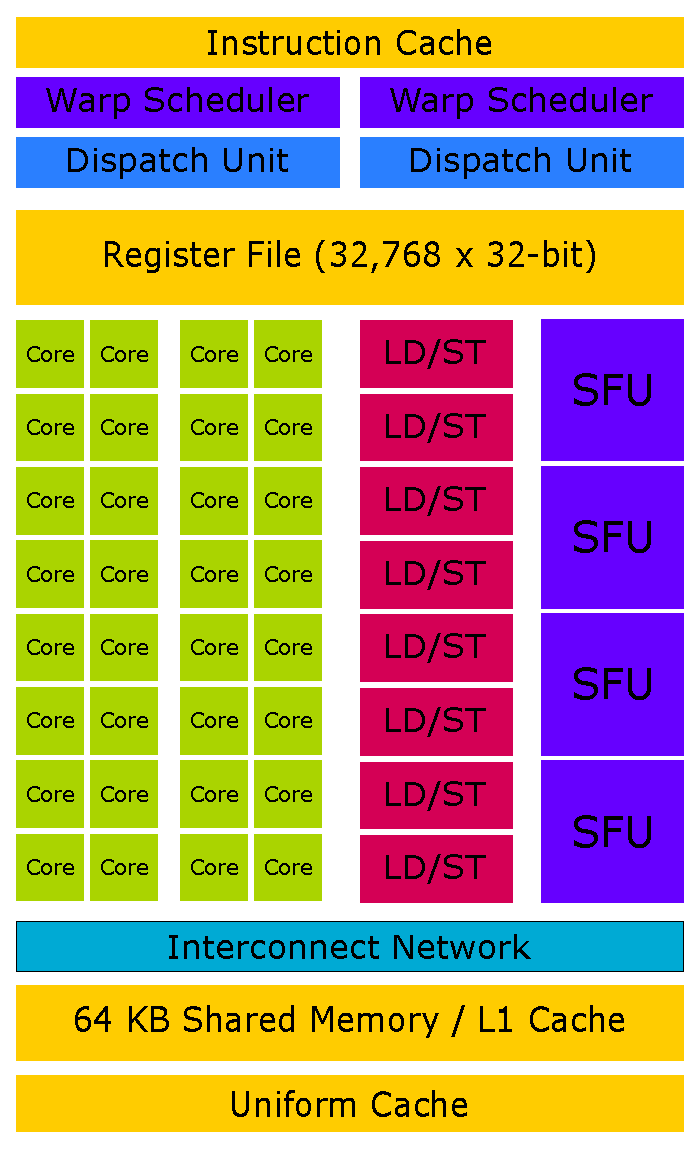
\includegraphics[width=0.8\linewidth]{img/SMPArchitecture.eps}
%  \caption{SMP architecture (Fermi)}
%  \label{fig:smparchitecture}
%\end{subfigure}
%\begin{subfigure}{0.6\textwidth}
  %\centering
  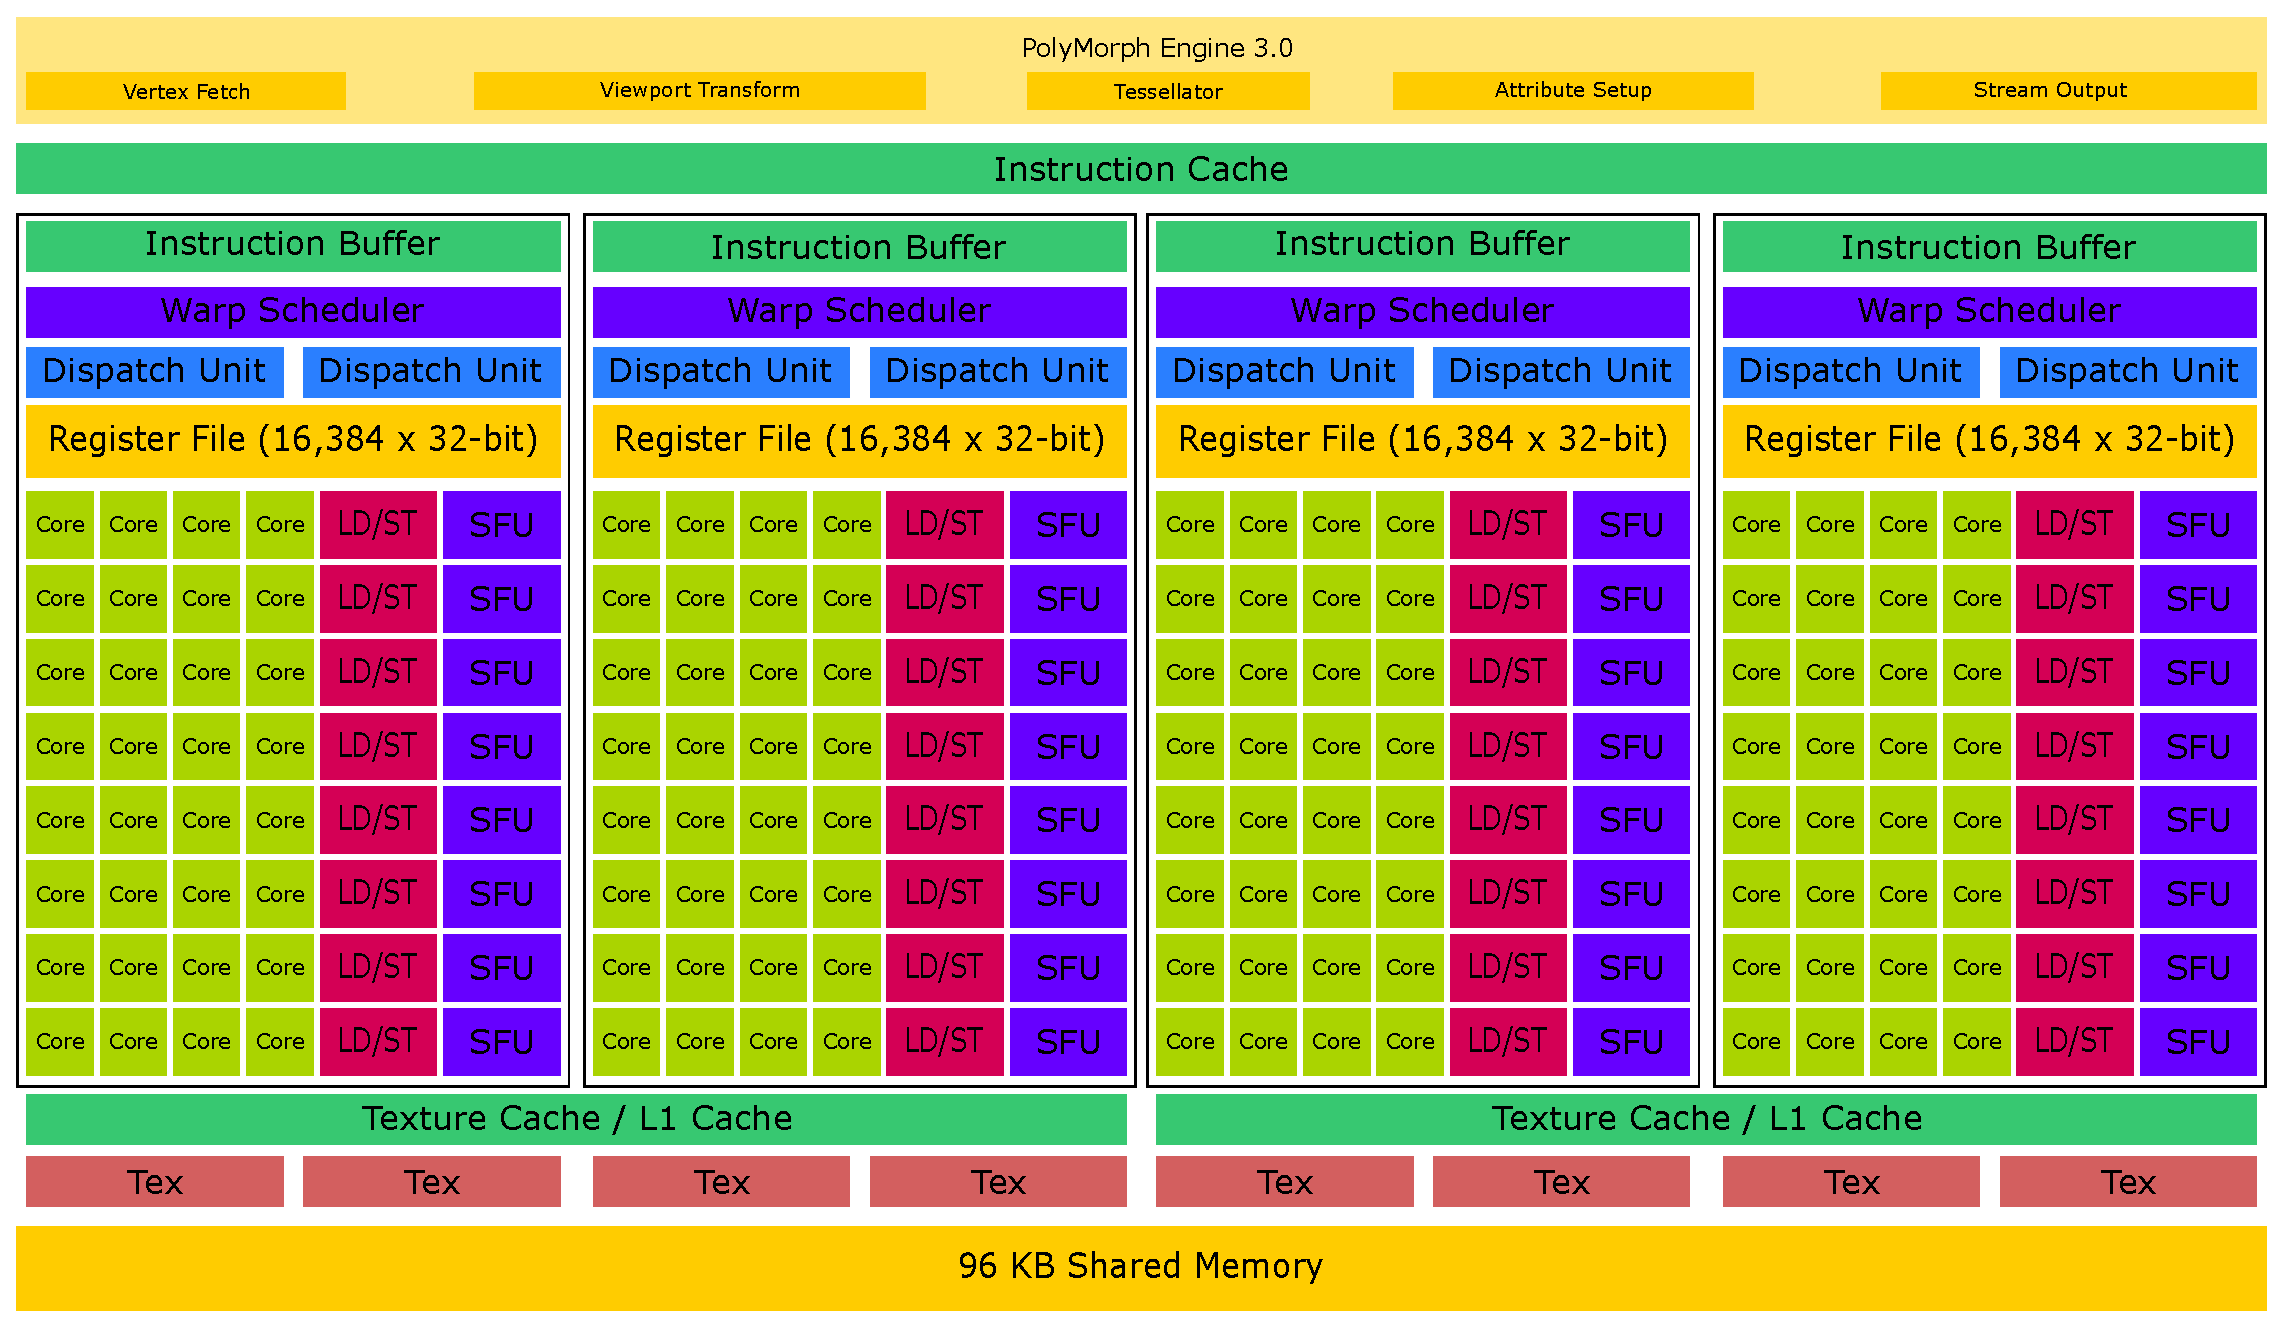
\includegraphics[width=1\linewidth]{img/SMMArchitecture.eps}
  \caption{SMM architecture (Maxwell)}
  \label{fig:smmarchitecture}
%\end{subfigure}
%\vspace*{0.1cm} 
%\begin{subfigure}{0.6\textwidth}
%  \centering
%  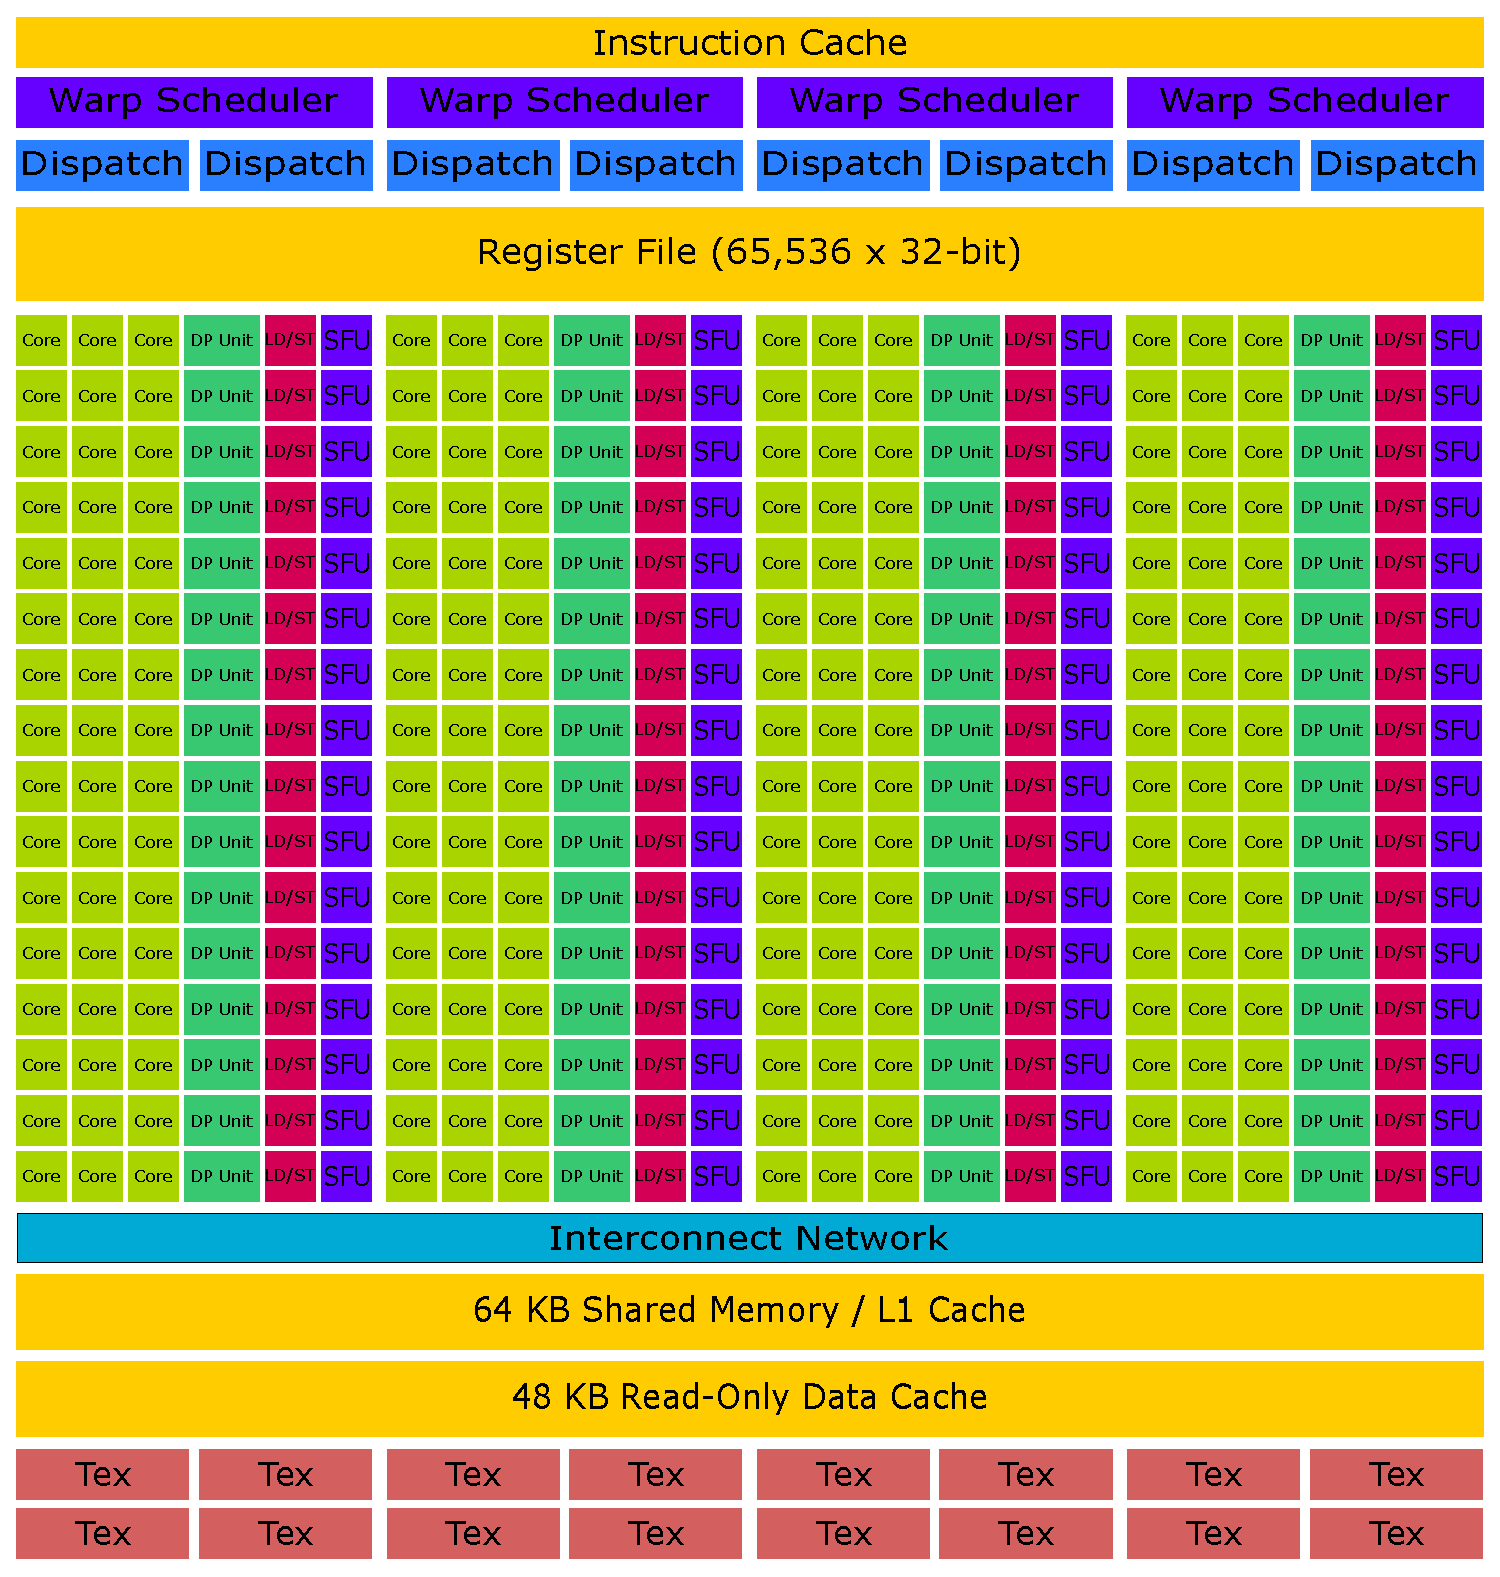
\includegraphics[width=0.9\linewidth]{img/SMXArchitecture.eps}
%  \caption{SMX architecture (Kepler)}
%  \label{fig:smxarchitecture}
%\end{subfigure}
\end{figure}

CUDA architecture contains larger processors called \textbf{Streaming Multiprocessor (SMP)}. The oldest is \textbf{SM} - Fermi, \textbf{SMX} - Kepler and the newest \textbf{SMM} - Maxwell~\autoref{fig:smmarchitecture}. Each SMP contains processor cores with registers (from 32 on Fermi architecture, 128 on Maxwell architecture and 192 on Kepler architecture), load/store units (LD/ST), Special Function Units (SFUs), shared instruction cache, shared memory and data caches. LD/ST and SFUs are shared by groups of cores, size of group depends on architecture.

\begin{figure}[h]
  \centering
  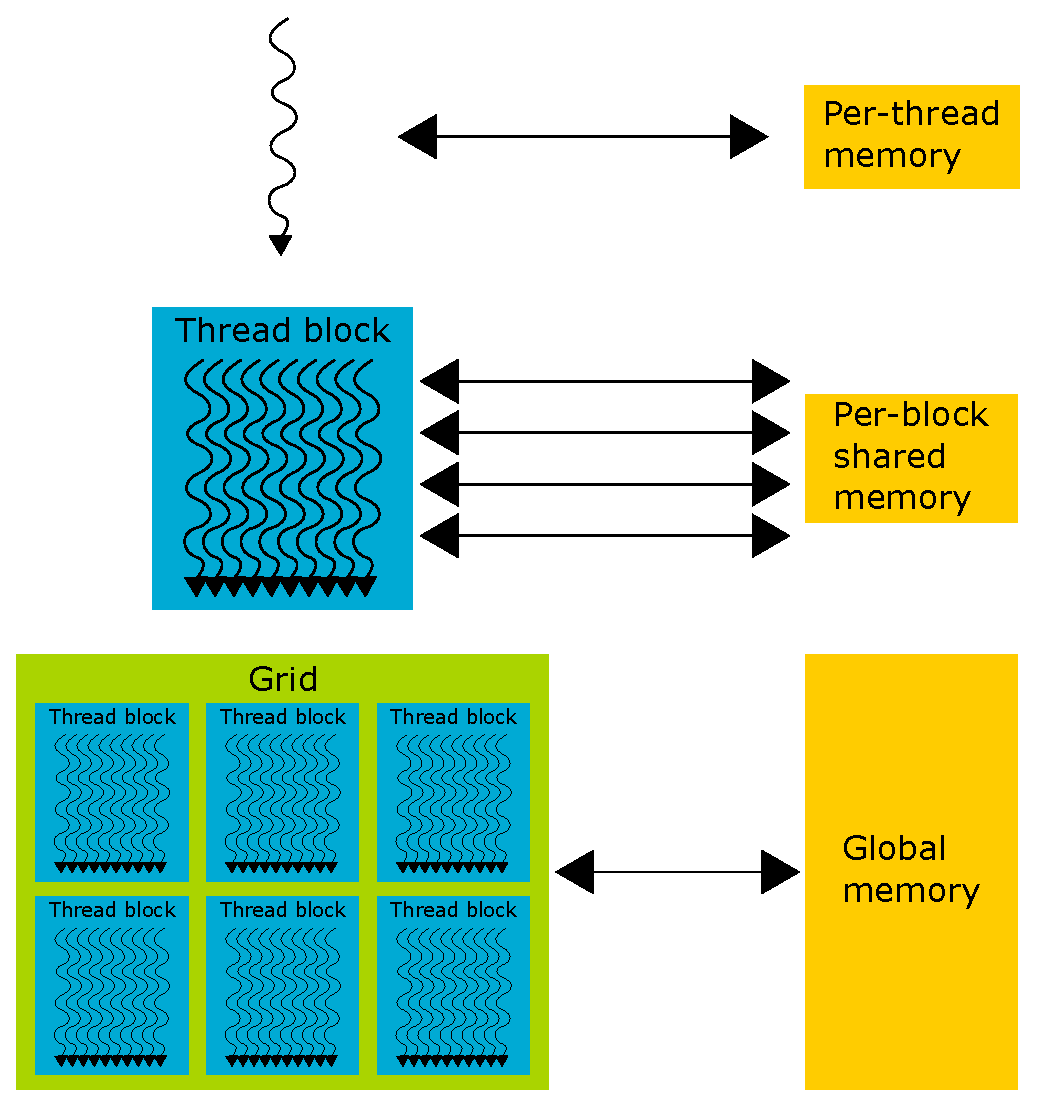
\includegraphics[width=0.8\linewidth]{img/CUDAmemoryHierarchy.eps}
  \caption{CUDA Execution model}
  \label{fig:cudamemhierarchy}
\end{figure}

Next different parameter of CUDA device is \textbf{Compute Capability} (CC), which describes the device characteristics and a set of instructions that are supported. CC is tightly coupled with architecture (CC 1.x was supported by Tesla architecture, CC 2.x by Fermi, 3.x by Kepler, 5.x by Maxwell).\\

CUDA use Simple Instruction Multiple Thread (SIMT) model. This model approaching parallelism by broadcasting same instruction to multiple execution units, so only one instruction fetch/decode unit is needed for group of execution units. This model is similar to Simple Instruction Multiple Data (SIMD) model, but the difference is that SIMT also have multiple register sets. Main difference is that SIMD processes short vectors in parallel and always all threads do the same work. For example, when we need sum two vectors, SIMD must iterate through vectors and in one step, it can only process as many elements as a computing units count is. On CUDA with SIMT model, we launch as many threads as size of vector and each thread can store values in own register.\\

\subsection{CUDA Workflow}
When we want to launch CUDA program, first think what we must do in host code is detect CUDA capable devices. When desired device is selected, we could start with copying data from host to device. This action is asynchronous so we must synchronize execution of host code and memory transfer. When data transfer is done, we could launch device code called \textbf{kernel}. Kernel is same as normal C function but defined with special declaration and it can use special device functions specified by CC. \\
Kernel is launched from host code same as normal function but it runs asynchronously. This function is executed $N$ times in parallel by different CUDA threads. Number of threads is specified at function call. Threads are arranged in one, two or three dimensional space so it could easily reflect data structures like vectors, matrices or volumes. This bunch of threads is called \textbf{block}. The number of threads in block is limited because all threads in block must reside on the same streaming multiprocessor and must share its limited memory resources so on current GPUs, maximum number of threads is 1024.\\
The total number of threads is multiplied by number of blocks. Blocks could be also arranged in one, two or three dimensional space. Only limitation is that each block must be equally shaped so usually the number of thread blocks is determined by size of data being processed or by total number of cores. The total number of threads which are executed in single kernel is number of threads times number of blocks as specified on~\ref{fig:cudagridthreadblock}. Kernel is also called asynchronously so when kernel is executing, host could for example start another memory transfer or doing another work on CPU. After synchronizing with device, we need usually transfer results from the device back to host which is again asynchronous call and must be synchronized.

\begin{figure}[h]
  \centering
  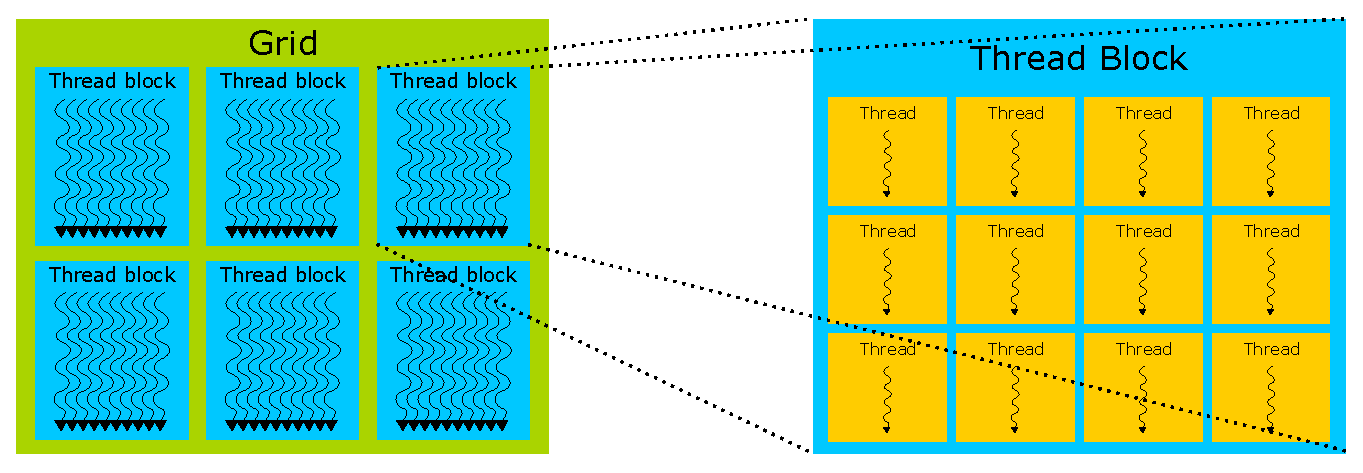
\includegraphics[width=1\linewidth]{img/CUDAthreadGridBlock.eps}
  \caption{2-dimensional grid of 2-dimensional thread blocks}
  \label{fig:cudagridthreadblock}
\end{figure}

Because number of cores is usually smaller than number of threads specified on kernel launch, only some threads could be run in parallel. These groups of threads are called \textbf{Warps}. When Kernel is launched, each block is assigned to SM and does not migrate to another SMP. Than, Each SMP splits its blocks into Warps depends on architecture. Warp threads are executed simultaneously by SMP cores. Splitting of the work between blocks and threads could significantly change the performance, because when we choose bad size of block (indivisible by Warp size) some Warps will not use all cores of single SMP. for example, if we launch same kernel with 8 blocks of 96 threads, block will be split into 3 warps which will be executed in parallel so we will have 24 warps to compute. Compare to that, if we launch the same kernel with 64 blocks of 12 threads, each block will be represented by warp containing only 12 threads so the total number of warps for execution will be 64 because CUDA is not capable to coalesce threads from different blocks. For this reason, it is recommended to set the size of the block to number divisible by size of Warp.\\
There are limitations for operations which could be run in parallel. For example, on Kepler architecture, only 4 of the 12 groups of cores can execute double precision operations at one time, so the slowdown of double precision computation may be up to 3 times. However, the other 8 groups could perform integer or float operations so the slowdown is usually smaller.\\
Problematic are problems with memory operations. Common CPU hides these latency by multilevel cache memory. CUDA architecture also contains some memory caches~\ref{fig:cudamemhierarchy} but because of the most common specialization of algorithms accelerated on GPU - stream or throughput computing, memory caching is ineffective. On CUDA, this is problem is reduced by more active warps on one core so when one warp stalls on memory operation, SMP switches to another ready warp. This mechanism keeps computing cores busy as possible and increasing the efficiency of computation.\\
Threads in single block are executed on a single SM. They share caches and could be synchronized across the threads from same warp. Compared to that threads from different Thread Blocks could be assigned to different SMPs or on same SMP concurrently. They could be even assigned to different or same SM at different times.

\subsection{Memory model}

Memory model on CUDA architecture~\ref{fig:cudamemaccess} contains more types of memory which differs mainly in size, bandwidth and latency.

\begin{figure}[h]
  \centering
  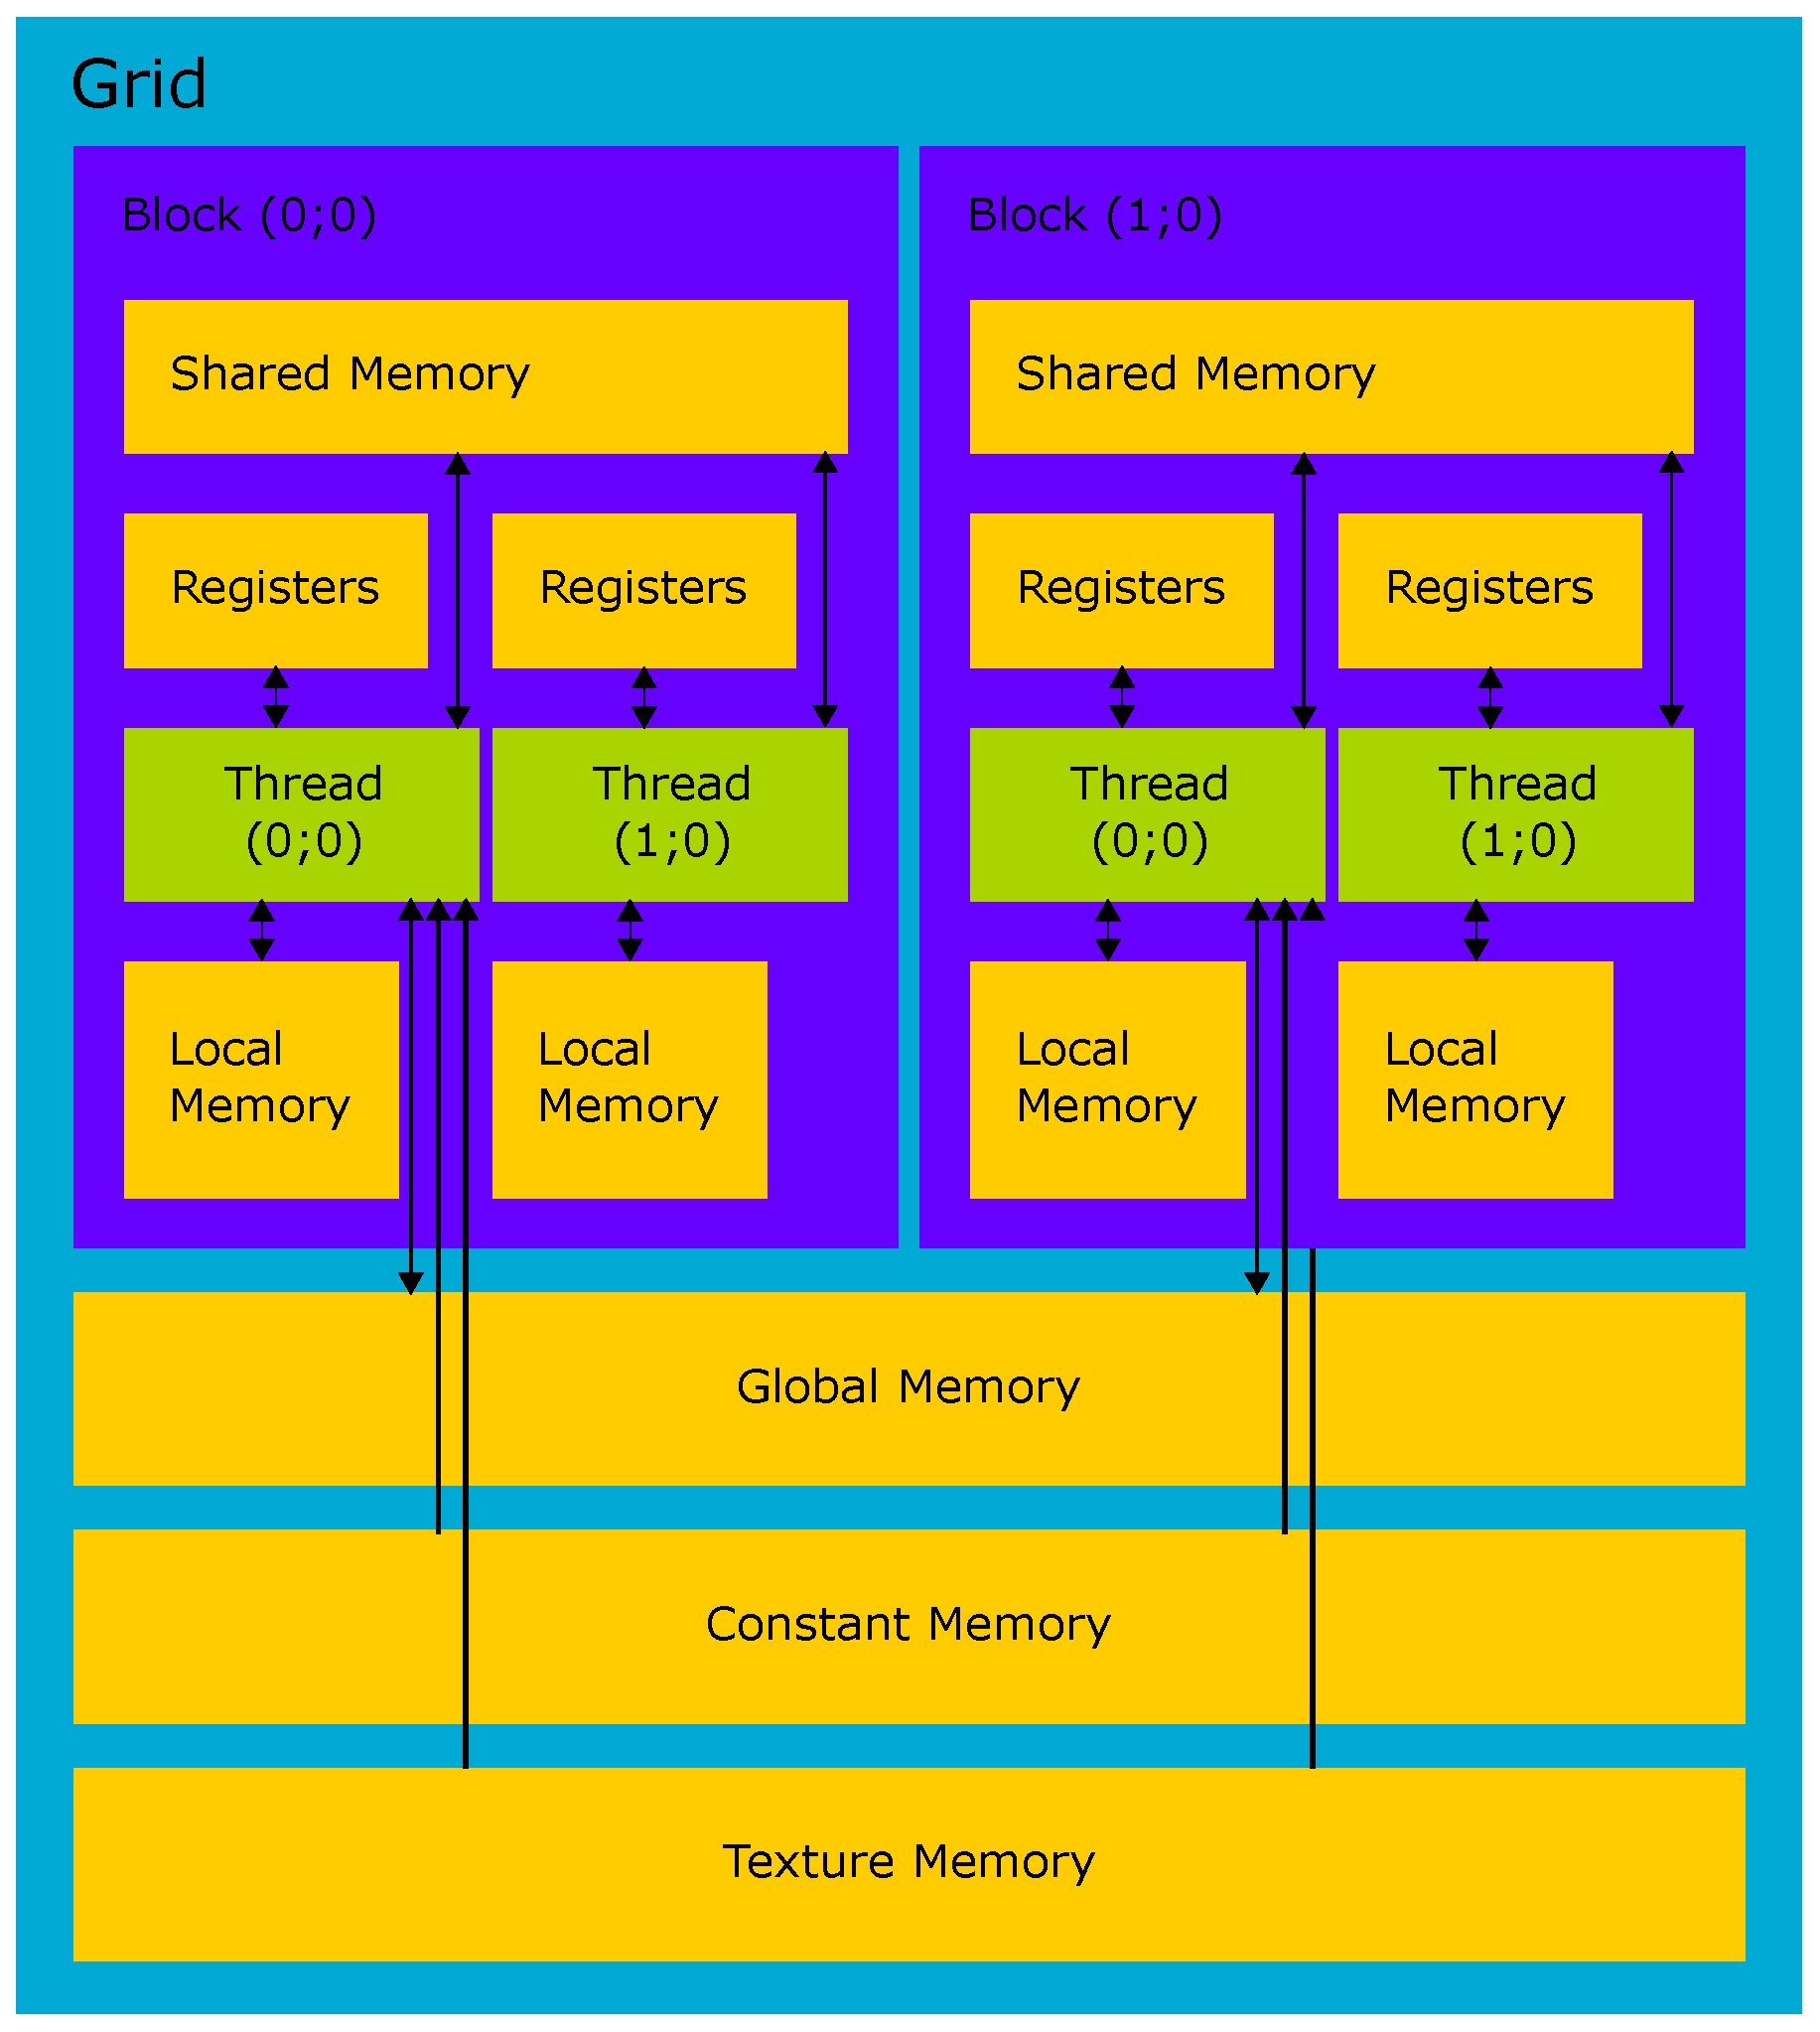
\includegraphics[width=0.6\linewidth]{img/CUDAmemAccess.eps}
  \caption{CUDA Memory access}
  \label{fig:cudamemaccess}
\end{figure}

\begin{description}
\item[Global memory] it is the largest memory (GBs) and it has high bandwidth (usually around 100 GBps) but high latency (400-600 clock cycles). It could be allocated eithe as CUDA arrays or as linear memory. CUDA arrays are opaque memory layouts optimized for texture catching. Linear memory exists on device in a 40-bit address space, so separately allocated entities ca reference another via pointers.~\cite{CUDAGuide} It is used for storing data transfered from host memory and it is allocated and released in host code by special CUDA API function before kernel launch. Global memory allocation is independent on kernel (except dynamically allocated memory inside kernel) and it could be used in many kernels without releasing and allocating new one for other kernel. Memory transfers are special host code CUDA API functions too, but they could be asynchronous. Same as memory allocation/deallocation, data are persistent between one kernel end and other kernel start. When data from this memory are accessed, they are cached in L2 cache. Also processed data or output is stored here before it is transfered back to host. It is operated in transactions of 32B - 128B so for better performance it is better to access data aligned on transaction size. Physically, it is off the chip, but on the device.

\item[Shared memory] is memory shared by all threads running on same SM. Shared memory has lower latency than global memory (32 bits / 2 cycles on CC 1.x and 2.x and 64 bits / 1 cycle on 3.x) than Global memory, but it is also smaller (depend on Compute Capability, from 16 kB on 1.x CC to 48kB on 2.x CC and 3.x CC). It could be as fast as registers if there are no bank conflicts. Shared memory has read-after write dependency which takes 24 clock cycles, but could be hidden by enough active warps. In shared memory are stored statically allocated variable or dynamic memory block could be allocated on kernel launch (it is one of kernel function parameters) and data are copied from global memory in kernel execution. Releasing of memory is done automatically after kernel is finished, so data stored here are not persistent between two kernels, they are even no persistent between same kernel re-execution.\\
This memory is divided into banks, each bank could be accessed independently which is really fast but if there are conflicts in accessing to same bank from multiple threads, access to the bank is serialized (except reading same address which is called broadcast) and could be many times slower, so for the best performance, it is better to avoid these conflicts (for example when threads accessing banks linearly~\ref{fig:linearaccess} or with stride~\ref{fig:strideaccess}, which is not a divisor of total banks count). On CC 1.x and CC 2.x, bank size is 32 bits, on CC 3.0 we can select between 32 bits and 64 bit banks. Physically it is situated near each processor for fast access.\\
\end{description}

\begin{figure}[h]
\centering
\begin{subfigure}{1.0\textwidth}
  \centering
  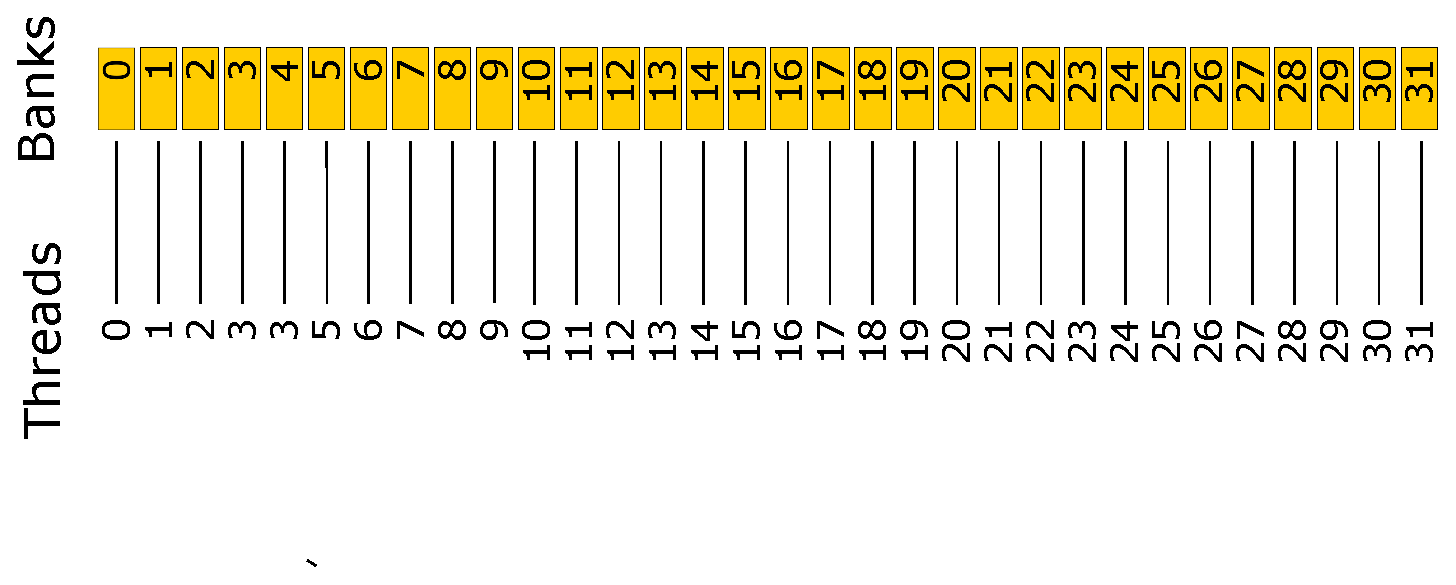
\includegraphics[width=.9\linewidth]{img/sharedMemoryLinearAccess.eps}
  \caption{Linear Access to shared memory}
  \label{fig:linearaccess}
\end{subfigure}
\begin{subfigure}{1.0\textwidth}
  \centering
  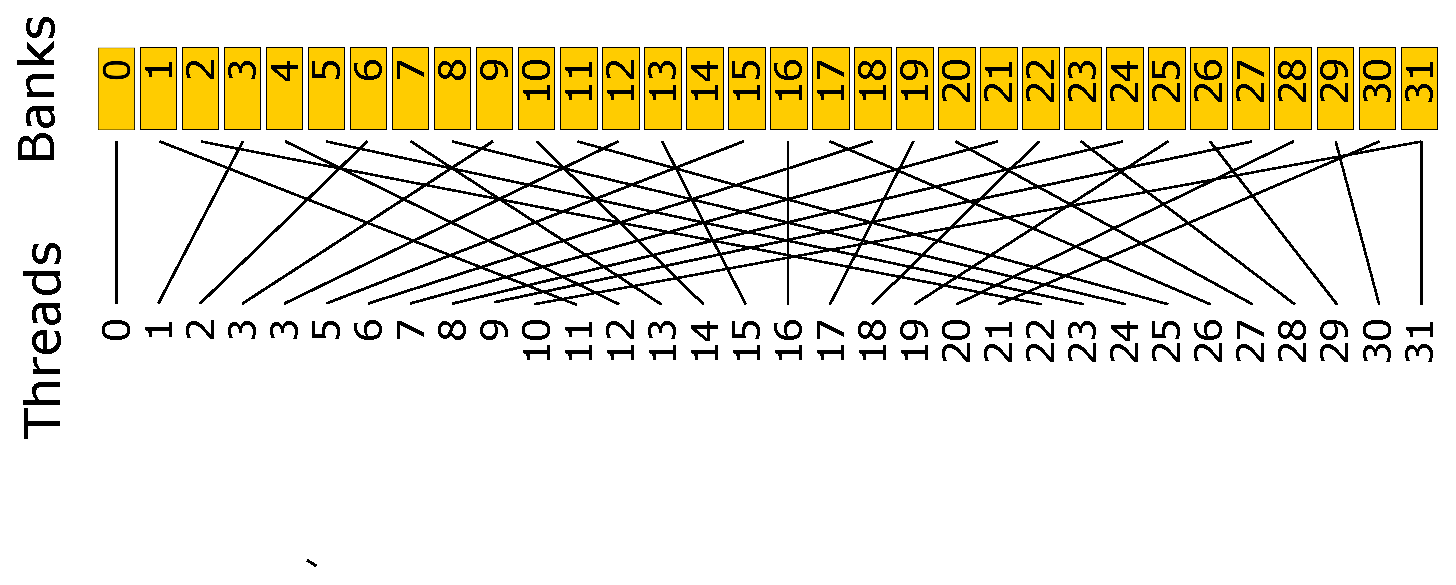
\includegraphics[width=.9\linewidth]{img/sharedMemoryStrideAccess.eps}
  \caption{Access to Shared Memory with stride 3}
  \label{fig:strideaccess}
\end{subfigure}
\caption{Shared Memory access}
\end{figure}

\begin{description}
\item[L1 Cache] has on most devices similar parameters as Share memory, because it has same resource. L1 cache is used for caching accesses to local and global memory so it could significantly speed up the memory access (100x-150x). We can configure which memory should be preferred and bigger by special CUDA API function from host code. On CC 5.0, L1 cache was merged with texture cache and is independent on shared memory (resources are not shared).
\item[Registers] Each multiprocessor has own register pool. Depend on CC, it has 8-64k of 32-bit registers. registers are the smallest memory, but also has the smallest latency (they are as fast as cores). For programmer, registers are not directly controllable. Only slow down is read-after write dependency, same as Shared memory, which takes 24 clock cycles, but it could be also hidden by enough of active warps. If kernel uses more registers than available, registers are stored to local memory. This problem is called \textit{registry spilling}.\\
Each thread has the same amount of registers. The number of registers per thread and the number of blocks determines, how many blocks could reside on SMP. For example, on CC 2.x, if kernel uses 32 registers and each block contains 512 threads, than two blocks can reside on SMP since they require $2*512*32$ registers, which exactly matches the number of registers available on SMP. If kernel uses one more register, than only single block could reside on SMP~\cite{CUDAGuide}.
\item[Local memory] is memory reserved in Global memory accessible by a single thread only. Only some automatic variables are stored in local memory~\cite{CUDAGuide}:
\begin{itemize}
\item Arrays for which it cannot determine that they are indexed with constant quantities,
\item Large structures or arrays that would consume too much register space,
\item Any variable if the kernel uses more registers than available (this is also known as register spilling).
\end{itemize}
Access to local memory are always cached by L1 and L2 memory on CC 2.x and CC 3.x. On CC 5.x, local memory accesses are always stored in L2 cache. 

\item[Constant memory] is a special memory for read-only data. Its size is 64kB and from CC 2.x, compiler stores here constant, thread-independent variables. From CC 2.x, compiler is forced to loading all constant, thread independent variables into this cache.
\item[Texture memory] is special memory used for graphics. Its benefit is 2D spatial locality used mainly for textures.
\end{description}

Data transfer between host and device are much slower than on device memory transfers (the limitation of PCI Express is 16/32 GBps depend on version, but could be slowed by host memory if the host memory is not fast enough or if source memory is swapped on disk). Memory transfer also take significant overhead, which could make CUDA inefficient for small data and compute inexpensive tasks. This problem could be solved by bulk transfers instead of individual memory transfers. Data transfer could be hidden by overlapping data transfer with computing, because CUDA device is capable of computing and simultaneously perform two asynchronous data transfers so for example, input data could be transfer for next computation step, kernel run and results from previous step could be transfered to host at one moment.\\
The host memory could be \textit{pinned} (or page locked) which could speed up memory transfer on systems with front side bus. \textit{Pinned memory} could be also used for \textit{Mapped memory} which allows eliminating memory transfers by mapping host memory into address space of device. All data transfers are than implicitly performed when data are needed by the kernel.

% is little bit different, because programmer can split execution of instructions into different branches by conditions based on thread identification. In both models